% !TeX spellcheck = en_US
\chapter{Model Unspecific Search in CMS}

The Model Unspecific Search in CMS (\emph{MUSiC}) is an analysis procedure that compares observed data to Monte Carlo (MC) expectations of the standard model. Unlike dedicated analyses that usually only regard a few decay channels, an unspecific search covers a broad spectrum of final states. Because MUSiC is sensitive to small deviations that occur in multiple decay channels, it is well suited for searches for processes that are not significant at low-energy scales.

This chapter will focus on the existing MUSiC workflow. First, the motivation behind an unspecific search will be illustrated, then the three steps \emph{skimming}, \emph{classification} and \emph{scanning} will be explained\cite{Pieta2012MUSiC,Papacz2014Model}.

\section{Motivation}
Since a Higgs boson candidate has been discovered at the LHC\cite{Ao2015Combined}, all predicted SM particles have been observed. Particularly in this time, questions about new physics beyond the standard model (BSM) arise. 
BSM phenomena include unification theories, heavy "copies" of the vector bosons (\PZprime, \PWprime), supersymmetric extensions to the SM (SUSY), string theories and quantum black holes.
Expected signatures of these models would show up in a large range of final states. For some models, narrow resonances are predicted, other result in a slight signature in the high-energy tail of the distributions.
The MUSiC analysis is sensitive to these kind of deviations.
Additionally, MUSiC can identify deviations between MC and data that originate from non-physics sources, uncovering weaknesses in the Monte Carlo simulation.

\section{Skimming}
The goal of skimming is to gather events from different data sources and convert them to a unified format containing only information relevant to MUSiC. AOD (analysis object data) files of observed as well as simulated events are downloaded from the computing grid to the local cache, where unnecessary information is stripped from the events. If the skimmed dataset originates from MC simulations, it is rescaled and shifted within its systematic uncertainties.
The resulting files are stored in the PXL I/O format\cite{BBE+2012Development}.

\section{Classification}
During the classification step, events are grouped into \emph{event classes} (EC) according to their physics content in the final state. 
Missing transverse energy is treated as separate physics object. There are three  types of event classes: \emph{exclusive}, \emph{inclusive} and \emph{jet inclusive}. Final states of events in exclusive event classes contain exactly the objects indicated in the event class name. 
Events in the exclusive EC \eventclass{1e + 1MET} contain only 1 electron and missing transverse energy in the final state, but no other physics objects.
Events in the inclusive EC can contain any other objects besides the indicated ones. \eventclass{1e + 1MET + X} contains at least 1 electron and missing transverse energy. 
Additionally, there are \emph{jet inclusive} event classes (e.g. \eventclass{1e + 1MET + Njet}), that exclusively contain the mentioned objects and zero or more jets, making the analysis more robust to initial and final state radiation caused by the emission of a gluon in the initial or final state.

These definitions imply that each event is contained in exactly one inclusive EC, at least one exclusive EC and at least one jet inclusive EC.

The classification algorithm automatically adjusts the possible event classes to the events actually contained in the dataset, spontaneously creating new classes. It also makes sure that events are only considered once, even if they have been stored by two separate triggers.

\subsection{Kinematic distributions}
For each event class, a histogram of the kinematic variables \sumpT, \Minv, \MET is calculated. The histograms are created with variable bin sizes according to the detector resolution\cite[p. 52]{Papacz2014Model}. Note that the vertical axis of histograms shown in this work carries the unit "Counts per \unit{10}{\GeV}", so to get the absolute number of events in a bin, the vertical data point has to be multiplied by the width of its bin.

% MUSiC/EventClassFactory/Resolutions.hh als Quelle
% Pauls Dis durchlesen
% AN: file:///T:/Temp/Downloads/AN2014_098_v5.pdf

\section{Scanning}
The scanning algorithm (\emph{scanner}) searches for the most significant deviation between MC and data in each histogram.

\subsection{Region Building}
For each histogram, the scanner probes all connected bin regions and calculates the \p value for each one.

The set of connected bin regions can be defined and calculated as
\begin{equation}
R = \{(s, e) \, \forall e \in (s + m, l) \, \forall s \in (0, l-m)\}
\end{equation}
where the histogram spans the bins $0$ to $l$ and $m$ denotes a minimal number of bins per region which can be configured.

For each region, the \p value is calculated. The region of most deviation (smallest \p) is called \emph{region of interest} and stored.

\subsection{The \p value}
The \p value expresses the probability of measuring a data point $\Ndata$ as significant as the one observed, or more significant, given the Monte Carlo expectation $\Nmc$.
Since the calculation deals with results of counting, experiments, a Poisson distribution is assumed. The probability of making an observation $N$ given the Poisson mean $\Nmc$ is
\begin{equation}
	P(N) = \frac{e^{-\Nmc} \Nmc^N}{N!}
\end{equation}
To include observations that are more extreme than the observation, the probabilities are summed away from the expectation:
\begin{equation}
p = 
	\begin{cases} 
		\displaystyle
		\sum\limits_{N = \Ndata}^{\infty} \frac{e^{-\Nmc} \Nmc^N}{N!} &\mbox{if} \; \Ndata \geq \Nmc \\
		\displaystyle
		\sum\limits_{N = 0}^{\Ndata} \frac{e^{-\Nmc} \Nmc^N}{N!} &\mbox{if} \; \Ndata < \Nmc
	\end{cases}
\end{equation}
Since the Poisson mean is usually not exactly known, for example because of Monte Carlo statistics, it is evaluated for multiple possible values $\theta$ which are weighted by a Gaussian distribution of width $\sigmamc$ around $\Nmc$. This final probability is called \emph{\p value}:
\begin{equation}
p = 
	\begin{cases} 
		\displaystyle
		\sum\limits_{N = \Ndata}^{\infty} C \cdot \int\limits_0^\infty \dd \theta \exp(-\frac{(\theta-\Nmc)^2}{2 \sigmamc^2}) \cdot \frac{e^{-\theta} \theta^N}{N!} &\mbox{if} \; \Ndata \geq \Nmc \\
		\displaystyle
		\sum\limits_{N = 0}^{\Ndata} C \cdot \int\limits_0^\infty \dd \theta \exp(-\frac{(\theta-\Nmc)^2}{2 \sigmamc^2}) \cdot \frac{e^{-\theta} \theta^N}{N!} &\mbox{if} \; \Ndata < \Nmc
	\end{cases}
\end{equation}
The constant $C$ denotes a normalization factor that compensates for using $0$ as the lower limit of the integral. This is necessary since the Poisson distribution with a negative expectation is not physical.

\subsection{The \ptilde value}
For a dedicated analysis looking at one fixed histogram region only, this \p value would be sufficient to describe the statistical significance of the deviation. But since the scanner algorithm regards many regions to choose the most significant one from, the probability of finding a deviation somewhere is larger than \p. This is called \emph{look elsewhere effect}.

To counter the look elsewhere effect, the scanning algorithm is applied multiple times on randomly diced pseudo-data. For each pseudo experiment, first the expected mean $\Nmc'$ is randomly diced from a Gaussian distribution around $\Nmc$, having the width of the systematic error $\sigmamc$. Taking this new pseudo-mean, a random Poisson number is chosen as new observed value $\Ndata'$. The dicing of pseudo experiments is performed in a correlated way, the choice of $\Nmc'$ is shared between all distribution in all event classes. The complete scanning algorithm is repeated for each pseudo-experiment, finding a region of interest and its \p value.
\begin{figure}[htbp]
	\center
	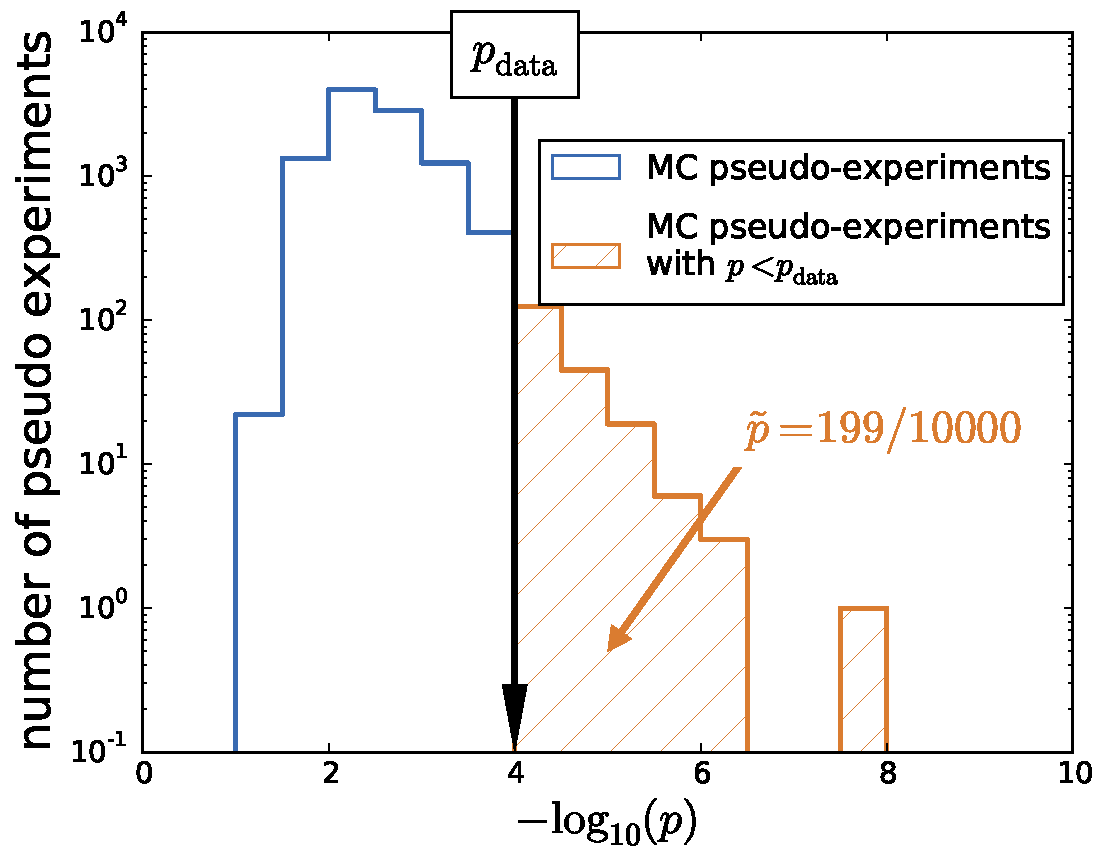
\includegraphics[width=0.6\textwidth]{ptilde_illustration.pdf}
	\caption{Illustration of a \ptilde calculation. 1000 pseudo-experiments have been conducted. The experiments on the right of $p_\mathrm{data}$ have shown a more extreme deviation somewhere in the distribution.}
	\label{fig:ptilde_illustration}
\end{figure}
Finally, the amount of pseudo experiments with more significant deviations is compared to the total amount of pseudo experiments conducted:
\begin{equation}
	\ptilde = \frac{\text{number of pseudo-experiments with } \p < \p_\mathrm{data}}{\text{total number of pseudo experiments}}
\end{equation}



